\documentclass[]{beamer}
% Class options include: notes, notesonly, handout, trans,
%                        hidesubsections, shadesubsections,
%                        inrow, blue, red, grey, brown

% Theme for beamer presentation.
\usepackage{beamerthemesplit} 
\usepackage[utf8]{inputenc}
\usepackage[T1]{fontenc}
\usepackage[english,swedish]{babel}
% Other themes include: beamerthemebars, beamerthemelined, 
%                       beamerthemetree, beamerthemetreebars  

\graphicspath{{figures/}{figures/hmm-graph/}{figures/gwhisker_database/}{figures/gwhiskers/}{figures/preprocessing}}

\renewcommand{\ae}{\"{a}}
\renewcommand{\oe}{\"{o}}
\renewcommand{\AE}{\"{A}}
\renewcommand{\OE}{\"{O}}

\newcommand{\prob}[1]{p\left(#1\right)}
\newcommand{\cprob}[2]{\prob{\left. #1 \middle\vert #2 \right.}}
\newcommand{\cprobnext}[1]{\cprob{#1_{n+1}}{#1_n}}
\newcommand{\ndist}[2]{\mathcal{N}\left(#1, #2\right)}
\newcommand{\norm}[1]{\left\|#1\right\|}
\newcommand{\Lp}[1]{\mathrm{L}^{#1}}
\newcommand{\bbset}[1]{\mathbb{#1}}
\newcommand{\RP}{\bbset{R}^+}
\newcommand{\ZP}{\bbset{Z}^+}

\title{Probabilistisk f\oe ljning av multipla morrh\aa r i monokul\ae r video}
\author{Jim Holmstr\"{o}m, Emil Lundberg}                 % Enter your name between curly braces
\institute{CSC,KTH}      % Enter your institute name between curly braces
\date{\today}                    % Enter the date or \today between curly braces

\begin{document}

% Creates title page of slide show using above information
\begin{frame}
  \titlepage
\end{frame}
\note{Talk for 30 minutes} % Add notes to yourself that will be displayed when
                           % typeset with the notes or notesonly class options

% slides are 3in high by 5in wide

\section{Introduktion}

\subsection{Bakgrund}
\begin{frame}
  \frametitle{Bakgrund}
  \begin{columns}[c]
    \column{2in}
    \begin{itemize}
    \item Neurofysiologer vill studera rörelser hos morrh\aa r
    \item Befintliga kommersiella l\oe sningar \ae r dyra eller kr\ae ver inskr\ae nkningar
    \item Hedvig Sidenbladh, 2001: probabilistisk metod f\oe r f\oe ljning av m\ae nskliga r\oe relser
    \end{itemize}
    \column{2in}
    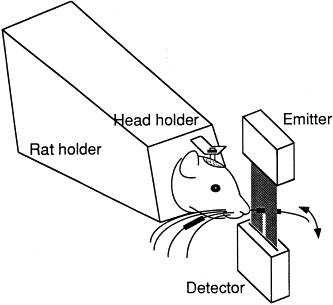
\includegraphics[width=0.75\textwidth]{optoelectronic.png}
  \end{columns}
\end{frame}

\subsection{M\aa l med projektet}
\begin{frame}
  \frametitle{M\aa l med projektet}
  \begin{itemize}
  \item Unders\oe ka om Sidenbladhs metod g\aa r att applicera h\ae r
  \item Testa n\aa gra olika varianter
  \item Identifiera problem och sv\aa righeter
  \end{itemize}
\end{frame}

\section[Agenda]{}

% Creates table of contents slide incorporating
% all \section and \subsection commands
\begin{frame}
  \tableofcontents
\end{frame}

\section{Probabilistisk metod}

\subsection{Dold Markovmodell}
\begin{frame}
\frametitle{Dold Markovmodell}
  \begin{columns}[c]
    \column{2in}
    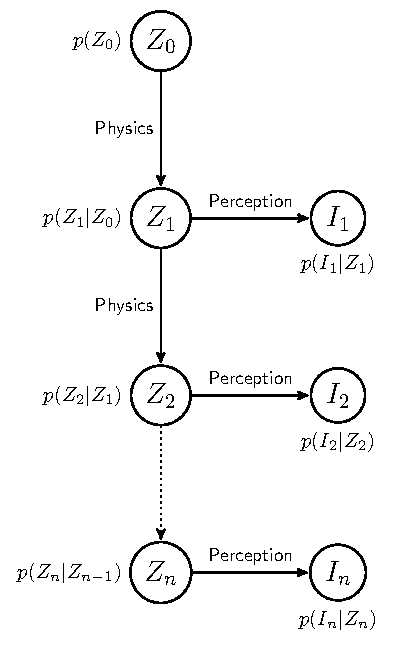
\includegraphics[width=0.8\textwidth]{hmm-graph.pdf}
    
    \column{2in}
    \begin{itemize}
    \item System \oe verg\aa r mellan tillst\aa nd med sannolikheter $\cprobnext{Z}$
    \item Tillst\aa ndet kan ej m\ae tas direkt
    \item F\aa r ist\ae llet en \emph{observation} $I_n$ av tillst\aa ndet $Z_n$ med sannolikhet $\cprob{I_n}{Z_n}$
    \end{itemize}
  \end{columns}
\end{frame}

\subsection{Partikelfiltret}

\begin{frame}
  \frametitle{Partikelfiltret}
  \begin{center}
    Approximerar sannolikhetsf\oe rdelning med diskreta m\ae ngder
    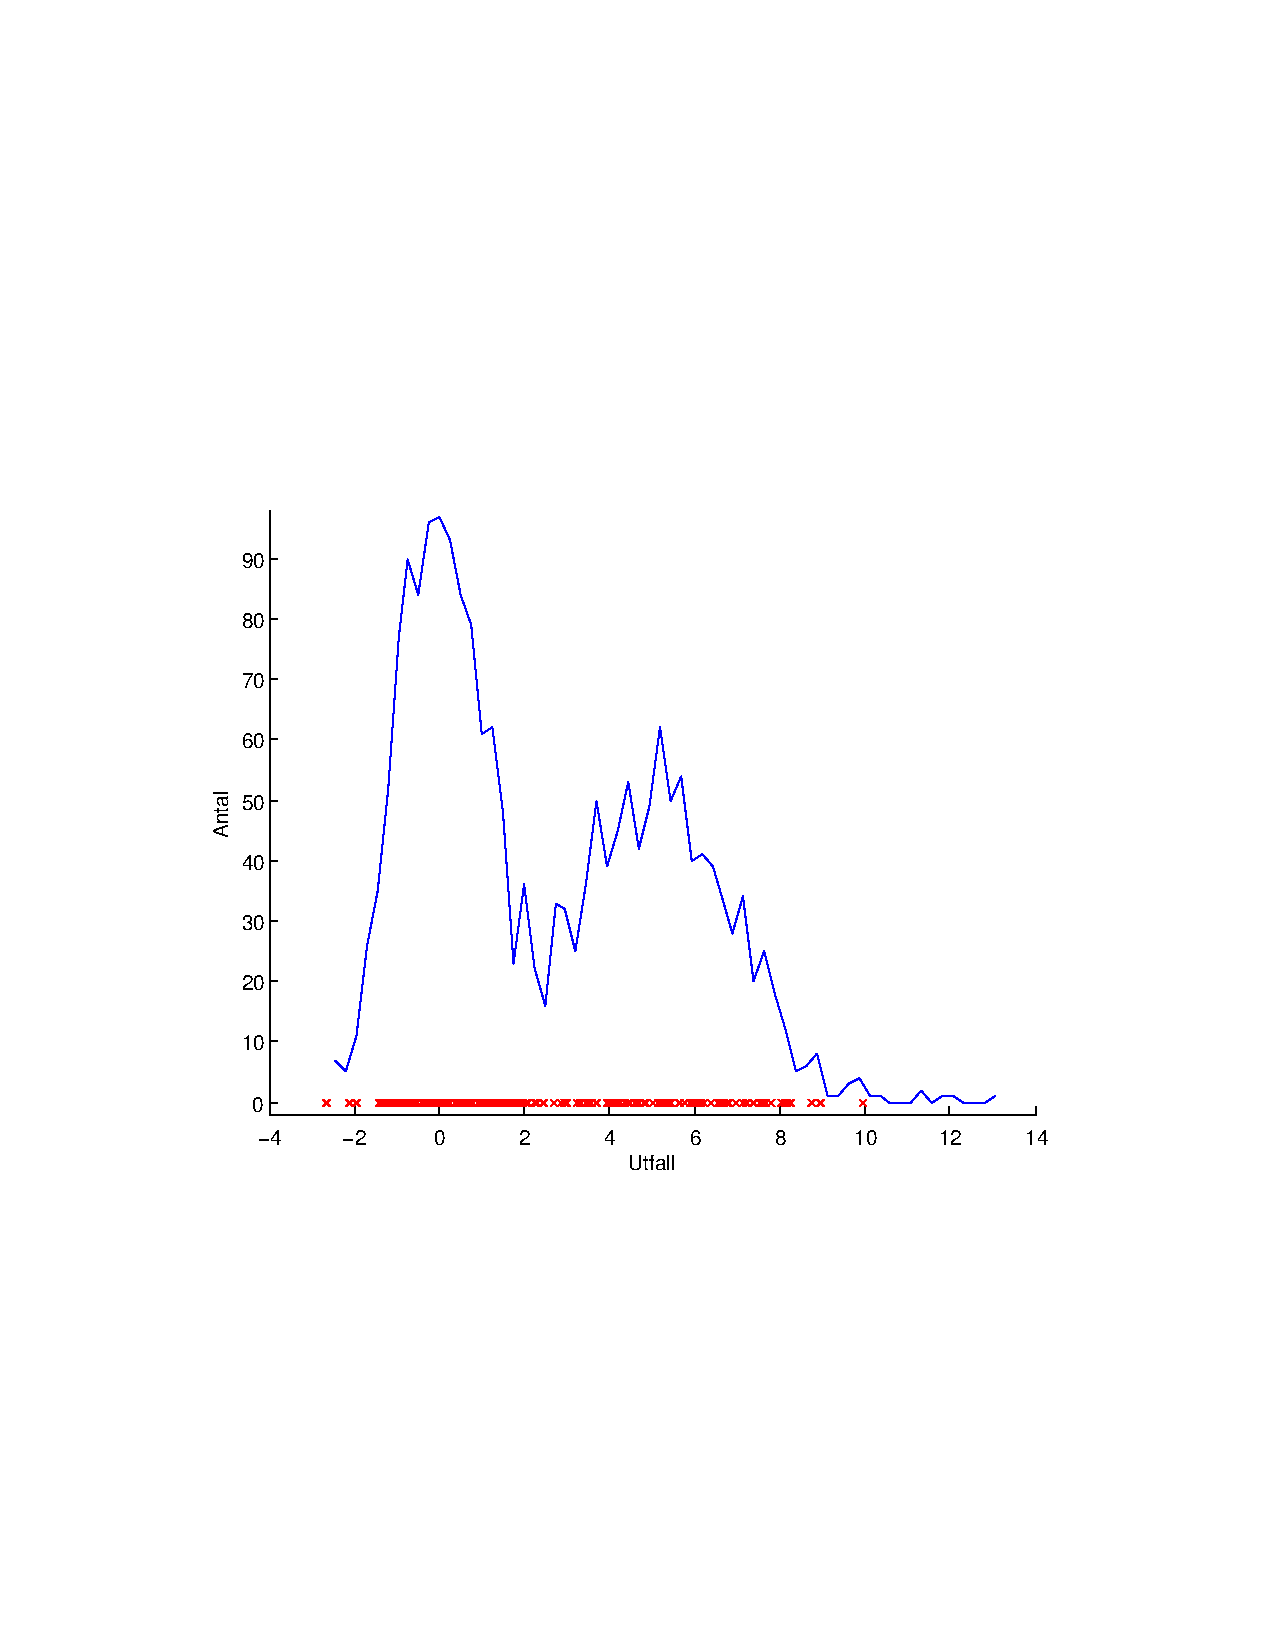
\includegraphics[trim=3cm 8cm 4cm 8cm, clip=true, totalheight=0.7\textheight]{hist.pdf}
  \end{center}
\end{frame}

\begin{frame}
  \frametitle{Partikelfiltrets fyra steg}
  \begin{columns}[tt]
    \column{2.5in}
    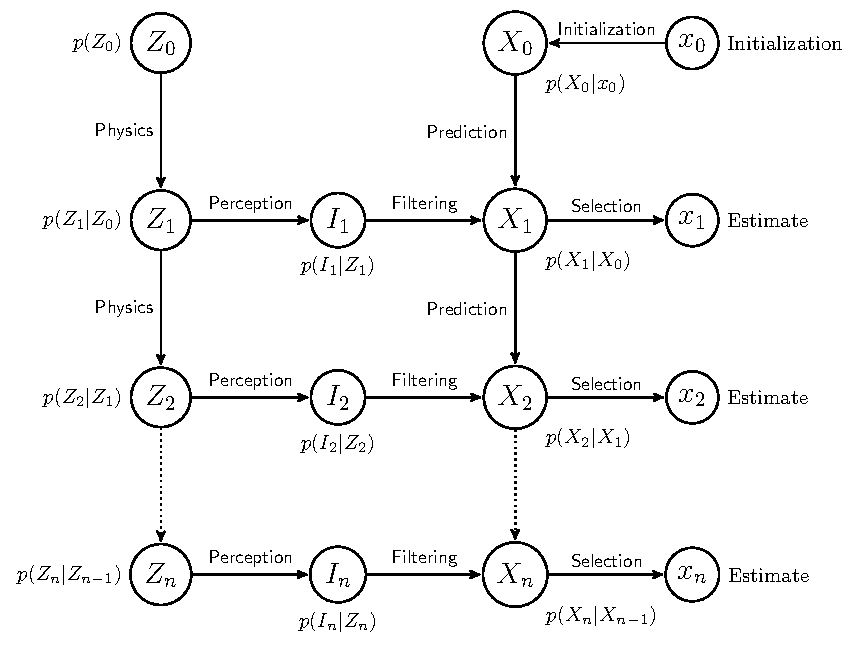
\includegraphics[width=1\textwidth]{hmm-graph-pf.pdf}

    \column{2.5in}
    \begin{description}
    \item[Prediktion] Skapa hypoteser om n\ae sta tidssteg
    \item[Perception] L\ae s in och tolka bild
    \item[Filtrering] V\ae lj ut de hypoteser f\oe r vilka bilden \ae r trolig
    \item[Urval] Konstruera en uppskattning av systemet utifr\aa n de filtrerade hypoteserna
    \end{description}
    
  \end{columns}
\end{frame}

\newcommand{\Circle}[1]{
  \begin{picture}(0, 0)
    \color{#1}
    \put(-16, 4){\circle{16}}
  \end{picture}
}
\newcommand{\Line}[1]{
  \begin{picture}(0, 0)
    \color{#1}
    \put(-24, 4){\line(1,0){16}}
  \end{picture}
}

\begin{frame}
  \frametitle{Illustration av stegen}
  \begin{columns}[c]
    \column{2.5in}

    \begin{description}
      \item[\Circle{blue}] F\oe re filtrering
      \item[]
      \item[\Circle{red}] Efter filtrering
      \item[]
      \item[\Circle{green}] Slutlig uppskattning
    \end{description}
    
    \column{2in}
    
    \begin{center}
      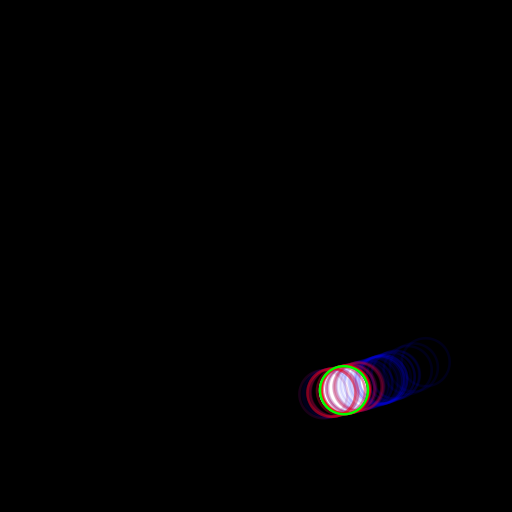
\includegraphics[width=1\textwidth]{pendulum-tracking.png}
    \end{center}
  \end{columns}
\end{frame}

\begin{frame}
  \frametitle{Illustration av stegen}
  \begin{columns}[c]
    \column{2.5in}

    \begin{description}
      \item[\Line{blue}] F\oe re filtrering
      \item[]
      \item[\Line{red}] Efter filtrering
      \item[]
      \item[\Line{green}] Slutlig uppskattning
    \end{description}
    
    \column{2in}
    
    \begin{center}
      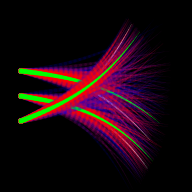
\includegraphics[width=1\textwidth]{tracking-particles.png}
    \end{center}
  \end{columns}
\end{frame}

\subsection{Morrh\aa rens Matematiska Modell}
\begin{frame}
  \frametitle{Morrh\aa rens Matematiska Modell}

  \begin{columns}[c]
    \column{3in}
    \begin{itemize}
    \item Mycket enkel modell: $a_1x + a_2x^2 + a_3x^3$
      \begin{itemize}
      \item Approximerar morrh\aa rens form inom felmarginal f\oe r blotta \oe gat
      \item Kan avvika lite i s\ae llsynta extrema fall
      \end{itemize}
    \item Andra kandidater t.ex. $\sum\limits_k a_k\sin \left(kx\right)$
    \end{itemize}
    
    \column{1.5in}
    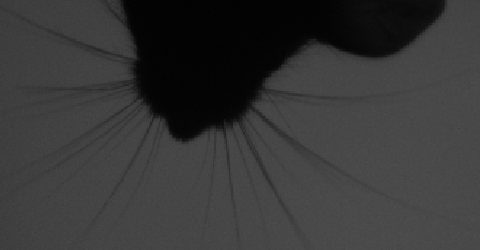
\includegraphics[width=1\textwidth]{rat-vanilla.png}

    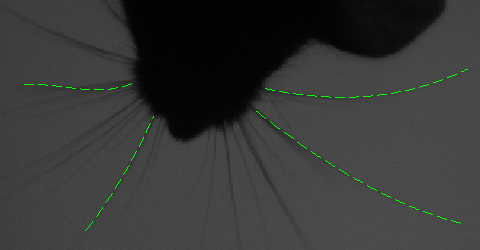
\includegraphics[width=1\textwidth]{rat-splines.png}
  \end{columns}
\end{frame}

\subsection{Prediktion: S\oe kning i databas med tr\ae ningsdata}
\begin{frame}
  \frametitle{Prediktion: S\oe kning i databas med tr\ae ningsdata}
  \begin{itemize}
  \item Implementerar $\cprobnext{X}$ som en s\oe kning i databas
  \item Databas av tillst\aa nds\oe verg\aa ngar $T = (f, t)$
  \item Givet en hypotes $x_n$ uppskattas $x_{n+1}$ som ett medelv\ae rde \oe ver $t$, viktat mot skillnaden mellan $x_n$ och $f$
  \item Viktfunktion $w(x_n, f)$
    \begin{equation*}
      x_{n+1} = \frac{\sum\limits_{(f, t) \in \mathrm{DB}} t \cdot w(x_n, f)}{\sum\limits_f w(x_n, f)} + \ndist{0}{\sigma}
    \end{equation*}
  \item T.ex. $w(x_n, f) = \norm{x_n - f}_{\Lp{p}}^{-a}$ f\oe r n\aa got $a\in \RP$
  \end{itemize}
\end{frame}

\begin{frame}
  \frametitle{Exempel\oe verg\aa ng}
  \begin{columns}[c]
    \column{2in}
    
\includegraphics[width=0.8\textwidth]{transition-example.png}
    
    \column{2in}
    \begin{itemize}
    \item Gul: Fr\aa n-tillst\aa nd
      \begin{itemize}
      \item $f = \frac{x^3 + 100x^2 - 2000x}{10000}$
      \end{itemize}
      
    \item R\oe d: Till-tillst\aa nd
      \begin{itemize}
      \item $t = \frac{x^3 + 150x^2 - 2000x}{10000}$
      \end{itemize}
    \item $\left(f, t\right) \in \mathrm{DB}$
    \end{itemize}
  \end{columns}
\end{frame}

\begin{frame}
  \frametitle{Exempel: Genererad databas}
  \begin{columns}[c]
    \column{2in}
    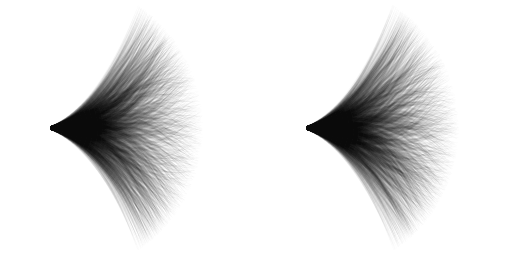
\includegraphics[width=1\textwidth]{database_gwhisker_spline3_n2048_from_to_fixed.png}
    
    \column{2in}
    \begin{itemize}
    \item Genererad databas av tillst\aa nds\oe verg\aa ngar
    \item V\ae nster: Fr\aa n-tillst\aa nd
    \item H\oe ger: Till-tillst\aa nd
    \end{itemize}
  \end{columns}
\end{frame}

\subsection{Filtrering: J\ae mf\oe relse av bilder}
\begin{frame}
  \frametitle{Filtrering: J\ae mf\oe relse av bilder}
  \begin{center}
    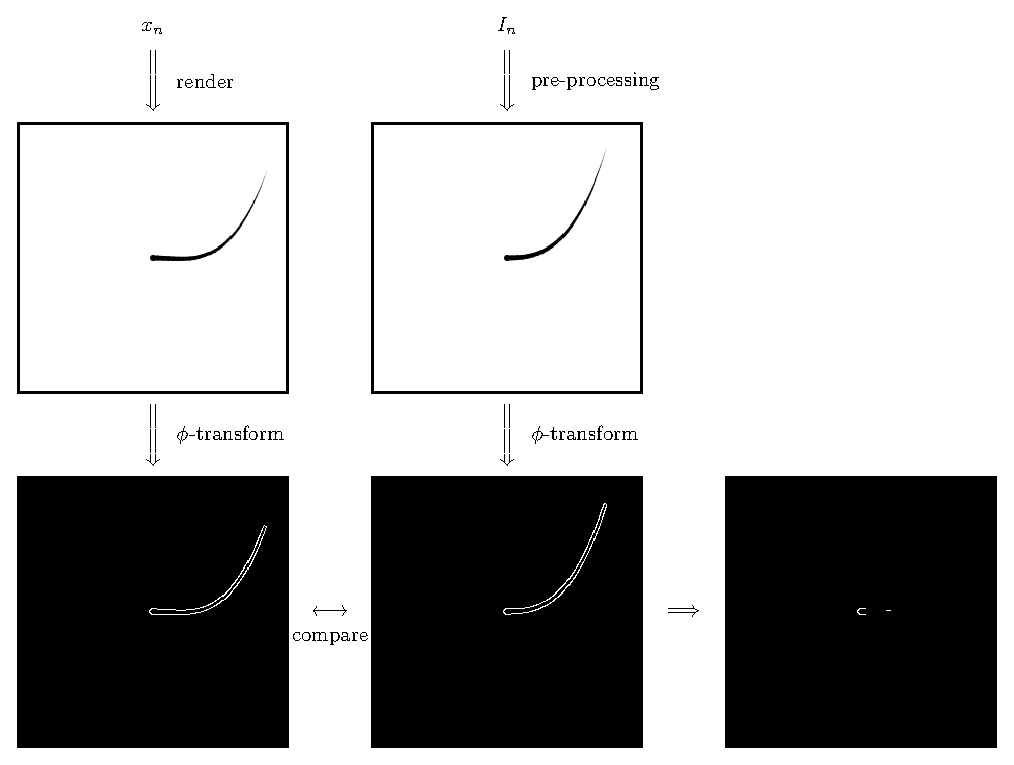
\includegraphics[width=0.8\textwidth]{whisker_compare.pdf}
  \end{center}
\end{frame}

\section{Resultat}
\begin{frame}
  \frametitle{Resultat: 32 partiklar, databas med 10000 \oe verg\aa ngar}
  
  \begin{center}
    \begin{tabular}{ccc}
      
\includegraphics[width=0.25\textwidth]{tracking/frame10.png}
      & 
\includegraphics[width=0.25\textwidth]{tracking/frame20.png}
      & 
\includegraphics[width=0.25\textwidth]{tracking/frame30.png}
      \\
      Bildruta 10 & Bildruta 20 & Bildruta 30\\
      
\includegraphics[width=0.25\textwidth]{tracking/frame40.png}
      & 
\includegraphics[width=0.25\textwidth]{tracking/frame50.png}
      & 
\includegraphics[width=0.25\textwidth]{tracking/frame60.png}
      \\
      Bildruta 40 & Bildruta 50 & Bildruta 60\\
    \end{tabular}
  \end{center}
\end{frame}

\begin{frame}
  \frametitle{Resultat: 256 partiklar, databas med 10000 \oe verg\aa ngar}
  
  \begin{center}
    \begin{tabular}{ccc}
      
\includegraphics[width=0.25\textwidth]{tracking-256/frame10.png}
      & 
\includegraphics[width=0.25\textwidth]{tracking-256/frame20.png}
      & 
\includegraphics[width=0.25\textwidth]{tracking-256/frame30.png}
      \\
      Bildruta 10 & Bildruta 20 & Bildruta 30\\
      
\includegraphics[width=0.25\textwidth]{tracking-256/frame40.png}
      & 
\includegraphics[width=0.25\textwidth]{tracking-256/frame50.png}
      & 
\includegraphics[width=0.25\textwidth]{tracking-256/frame60.png}
      \\
      Bildruta 40 & Bildruta 50 & Bildruta 60\\
    \end{tabular}
  \end{center}
\end{frame}

\begin{frame}
  \begin{itemize}
  \item Resultaten p\aa\ genererade morrh\aa r verkar lovande
    \begin{itemize}
      \item F\oe rv\aa nansv\aa rt bra resultat med endast 32 partiklar
      \item Mycket litet fel med 256 partiklar
      \end{itemize}
  \item \AA terst\aa r att g\oe ra:
    \begin{itemize}
    \item Testa p\aa\ riktiga morrh\aa r
    \item Optimera parametrar (bl.a. $a$ och val av $\Lp{p}$)
    \end{itemize}
  \end{itemize}
\end{frame}

\section{N\ae sta steg}
\begin{frame}
  \frametitle{N\ae sta steg}
  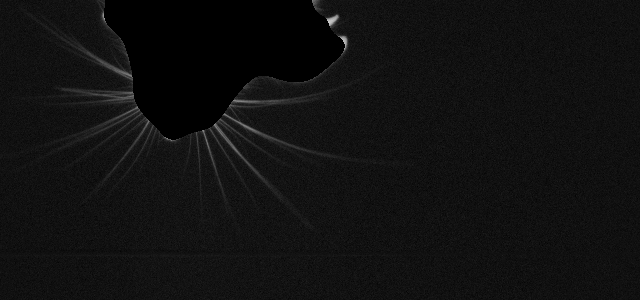
\includegraphics[width=1\textwidth]{preprocessing/frame-0759_whiskers.png}
\end{frame}

\end{document}
